\section{View}
\label{view}
This section deals with the various aspects of implementing the view layer of the GIRAF MVC architecture in GIRAF-W-11. The applied web technologies, the structural composition of the views (both visually and ond disk) and the interpretation of MVC in this scope will be described with the intention of creating a comprehensive understanding of the views in GIRAFAdmin.

\subsection{Technology}
As GIRAFAdmin is web-based, the most obvious choice for implementing viwes are through the de facto standards of (X)HTML and CSS. Apart from this, using JavaScript (notably with the JavaScript library \emph{jQuery}) offers more reactive web pages that can be made to only reload partially instead of completely reloading the page on every new request. See chapter \vref{implementation_tools_languages} for an introduction to the various tools and concepts.

The following figure depicts the most predominant output of the current implementation and the views and segments it is split into. Note in particular the header and footer of the page (much of it invisible to the user as it merely sets up the environment), which can be re-used in other views to create a global style and functionality on the site. The division is made from a conventional divide and conquer methodology. By solving the issue of CSS style and JavaScript inclusions in one place, they can easily be upgraded or switched out in one place while still affecting the entire site. Conversely, removing the redundancy from all "content" views (views with the actual content or representations of the model) makes for a cleaner base template for views and their interchangeability.

\begin{figure}
    \begin{center}
    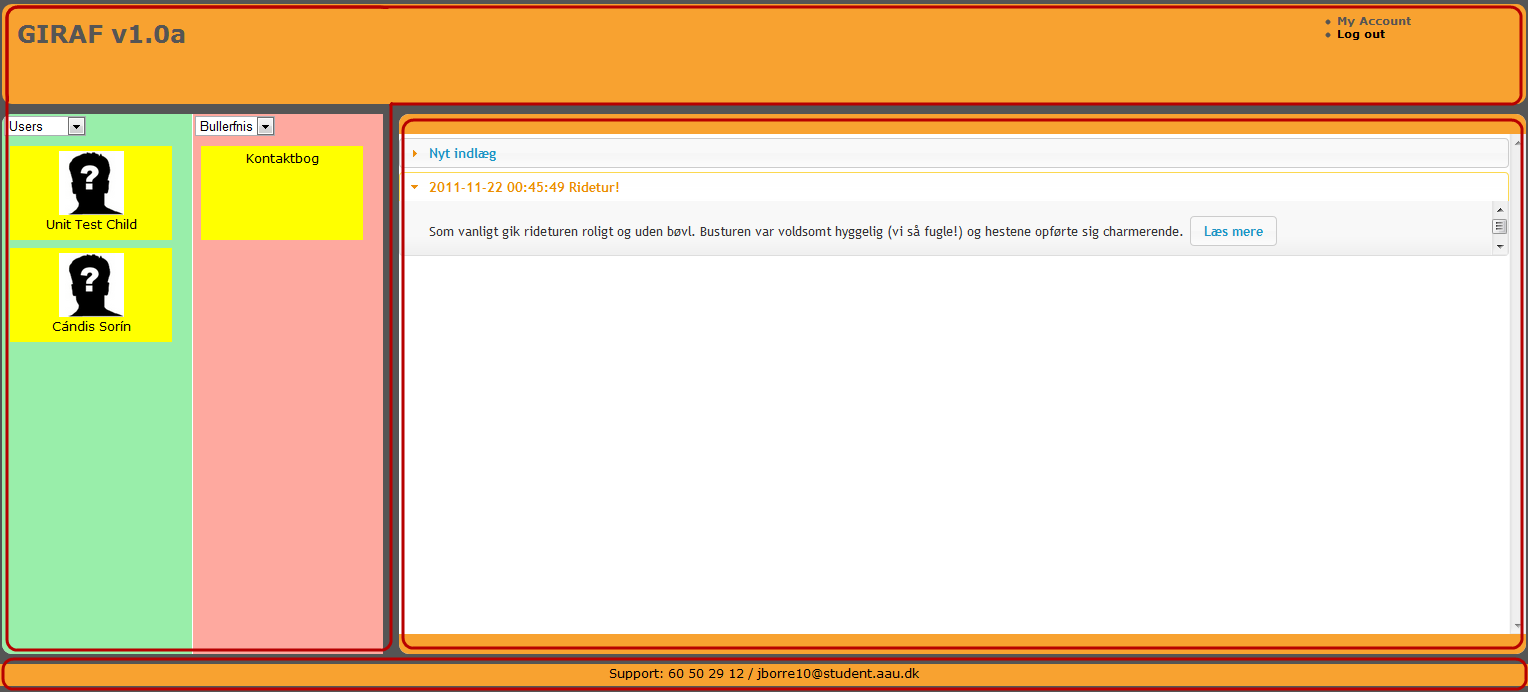
\includegraphics[scale=0.45,angle=90]{img/mvc_details/mvc_detailed_views}
    \caption{\label{implementation_view_views1}The red boxes show distinct views that have been loaded into the page. The one view invisible to the user is the header, loaded before any content.}
    \end{center}
\end{figure}

\begin{figure}
    \begin{center}
    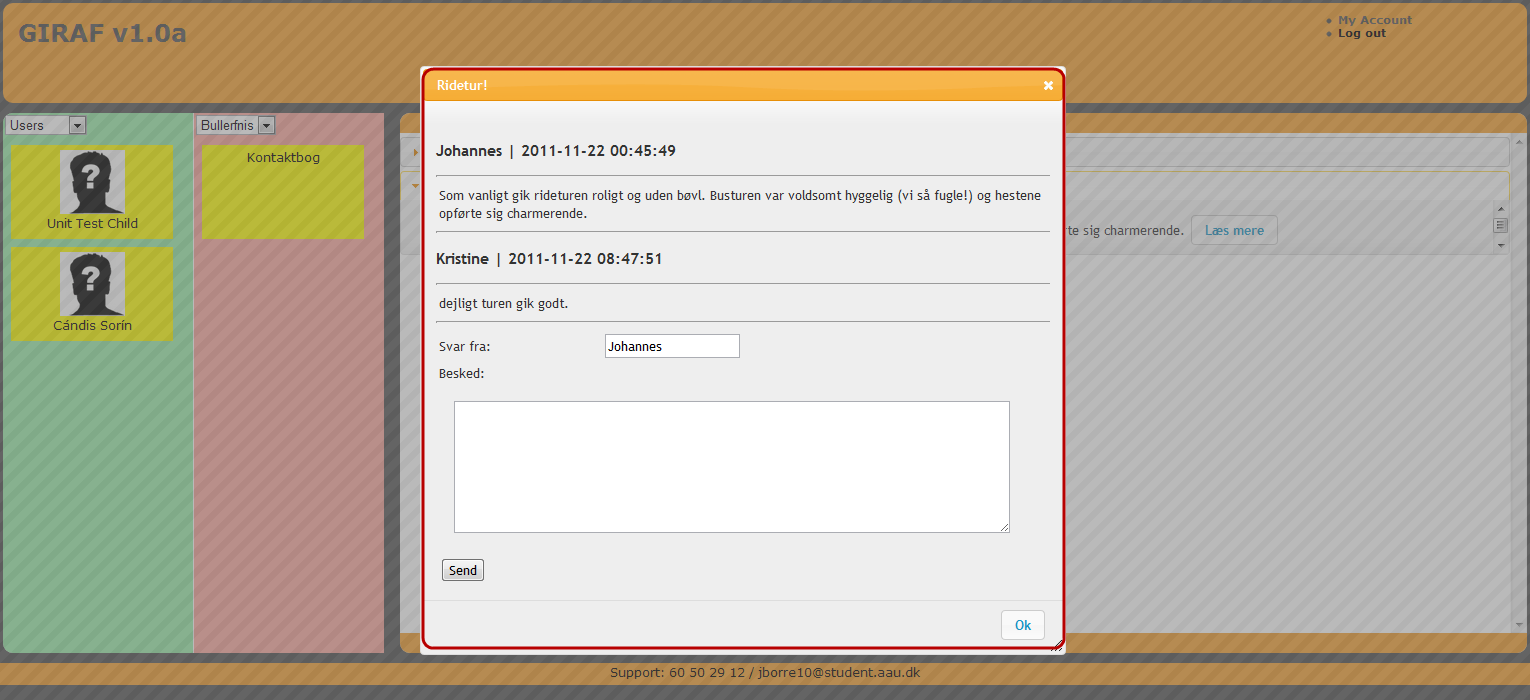
\includegraphics[scale=0.45,angle=90]{img/mvc_details/mvc_detailed_views2_view}
    \caption{\label{implementation_view_views1}The red box displays an extra view brought in by \emph{Contactbook}.}
    \end{center}
\end{figure}

The views in MVC represent everything that is displayed to the end user. There is some leeway in the pattern specification as to how the view is accessed. GIRAFAdmin follows a method used by several MVC frameworks where the view is invoked and displayed by the controllers after user input has been parsed and interpreted. Each view is a PHP script file. By this virtue there is no requirement that the output be HTML - a controller for listing users in the GIRAFAdmin database could as well output a full web page as it could output a PDF file generated by LaTeX or JSON data for cross-site API usage - the latter is actually an output format used to implement AJAX in the main view to deliver a more reactive user interface.

\subsection{Structure}
View files are placed in the \emph{/views} directory where they can be invoked by a controller using the \emph{view} method. Views specific to GIRAF applications (such as the contact book) should be placed in uniquely named subdirectories in the \emph{/apps} folder. Core views for GIRAFAdmin are placed in \emph{/default}.
As noted earlier, views are separated into three parts: header, footer and content. Implementing global header and footer views makes it a simple matter to quickly change the global style of the entire site or inject content into documents that already have defined header sections. In fact, although sub controllers like \emph{Contactbook} are injected into the content view \emph{main\_stub}, this approach allows for the sub controllers to be displayed by themselves simply by prepending a header and appending a footer, resulting in a very flexible view structure.
Although views can, in principle, perform the same actions as controller and model (as there is no scope or script restrictions) it is highly discouraged. Instead, views should rely solely on the output functions of PHP and the variables initialized by the calling controller. When a view is invoked, it is passed (by value) a set of variables from the controller and is implemented to display or discard data as necessary for final output to the calling environment.

\subsection{Code}
Views have no governing base class like the model's \emph{GirafRecord} or controller's \emph{GirafController}. Instead, each view file should be specifically tailored within its domain and role. All currently implemented views, for example, are written in the header-content-footer style, outputting HTML for display in browsers.
Creating new views has to be done within the purview of new or existing controllers. A view cannot be displayed without a controller to pass on relevant information from the model's current state. While not impossible, it is more likely that new views will be introduced to controllers than two different controllers will invoke the same view.

\subsection{Current views}
In its current iteration, GirafAdmin has six views. A single header (header.php), footer (footer.php) and four content views, login, main (main\_stub) and two views for the contact book, list and show. While each content view expects the header to be loaded, they are completely independent otherwise. This means that although \emph{Contactbook} is loaded inside of main\_stub, it can just as easily be displayed on its own.
